\documentclass[11pt]{article}

\usepackage{amsmath}
\usepackage{amssymb}
\usepackage[margin=0.68in]{geometry}
\usepackage{booktabs}
\usepackage{enumitem}
\usepackage{fancyhdr}
\usepackage{graphicx}
\usepackage[table]{xcolor}
\usepackage[hidelinks]{hyperref}
\usepackage{listings}
\usepackage{microtype}
\usepackage{tabularx}
\usepackage{titlesec}
\graphicspath{{docs/lessons/assets/}{../assets/}}

\definecolor{Ink}{gray}{0}
\definecolor{CodeGray}{gray}{0.96}
\hypersetup
{
    pdftitle={ADK Lesson 026: Telemetry Packet Evidence},
    pdfauthor={Kevin Shanahan},
    pdfsubject={Bounded telemetry packets, integrity, sequence, freshness, and visible evidence},
    pdflang={en-US}
}
\pagestyle{fancy}
\fancyhf{}
\lhead{\textsc{ADK Lesson 026}}
\rhead{Telemetry Packet Evidence}
\cfoot{\thepage}
\setlength{\headheight}{14pt}
\setlength{\parindent}{0pt}
\setlength{\parskip}{5pt}
\setlist{nosep,leftmargin=1.45em}
\titleformat{\section}{\Large\bfseries\color{Ink}}{\thesection}{0.5em}{}
\titleformat{\subsection}{\large\bfseries\color{Ink}}{\thesubsection}{0.5em}{}
\lstdefinestyle{adkcpp}
{
    language=C++,
    backgroundcolor=\color{CodeGray},
    basicstyle=\ttfamily\small,
    keywordstyle=\color{Ink}\bfseries,
    commentstyle=\color{Ink},
    columns=fullflexible,
    keepspaces=true,
    showstringspaces=false,
    frame=single,
    rulecolor=\color{Ink},
    breaklines=true,
    tabsize=4
}
\newcommand{\checkbox}{\(\square\)}
\newcommand{\blank}[1]{\rule{#1}{0.4pt}}
\newcommand{\lessonbox}[1]{%
  \begin{center}
  \fcolorbox{Ink}{white}{\parbox{0.92\linewidth}{#1}}
  \end{center}}

\begin{document}

\begin{center}
  {\Huge\bfseries Telemetry Packet Evidence}\\[4pt]
  {\Large Verify bytes before trusting an observation}\\[8pt]
  \textit{A local fixture makes integrity, sequence, and age visible.}
\end{center}

\begin{tabularx}{\linewidth}{@{}>{\bfseries}l X >{\bfseries}l X@{}}
Lesson & 026 --- component & Time & 150--210 minutes\\
Prerequisites & Lessons 001--025 & Board & Arduino Mega 2560\\
Primary evidence & D45 / TP-LED & Status & host verified; bench open\\
Safety boundary & E1, compiled-in fixtures, no radio receiver or transmitter\\
\end{tabularx}

\section{Mission}

Preserve the evidence chain:
\[
\text{packet bytes}\rightarrow\text{integrity}\rightarrow
\text{accepted observation}\rightarrow\text{local age}\rightarrow
\text{visible cadence}.
\]
\texttt{TelemetryPacketCodec} defines one exact bounded ADK lab packet.
\texttt{ObservationTracker} makes sequence and local freshness explicit.
This packet is not an observed radio protocol. The canonical sketch creates
its fixtures locally and neither receives nor emits RF.

\lessonbox{\textbf{Integrity is not trust.} CRC-16 detects accidental changes.
It does not authenticate a sender, hide a payload, prove provenance, prevent
replay, or make an unknown capture lawful to retain.}

\subsection{Learning outcomes}

\begin{itemize}
  \item distinguish packet, sample, observation, and record;
  \item explain exact-length decoding and unchanged output on failure;
  \item classify first, in-order, duplicate, gap, and reordered sequence values;
  \item calculate freshness from local receipt time rather than a remote clock;
  \item separate transport corruption, sample quality, and staleness;
  \item prove acquisition and safe state with separate circuit evidence.
\end{itemize}

\section{Parts, energy, and wiring}

\begin{tabularx}{\linewidth}{@{}l X@{}}
\toprule
Part & Requirement\\
\midrule
Arduino Mega 2560 & USB-powered board\\
Evidence LED & One ordinary LED and one 1 k\(\Omega\) resistor\\
Instrument & Logic probe or oscilloscope; meter for static safe-state check\\
Fixtures & Compiled-in ADK-owned bytes; no external receiver\\
\bottomrule
\end{tabularx}

For an illustrative 5 V rail and 2 V LED drop,
\[
I=\frac{5\text{ V}-2\text{ V}}{1000\ \Omega}=3\text{ mA}.
\]
Measure the actual rail, resistor, and LED drop before recording current.
Remove USB power before changing wires or probe clips.

\begin{tabularx}{\linewidth}{@{}l l X@{}}
\toprule
Signal & Mega pin & Connection\\
\midrule
Acquisition evidence & D13 & built-in LED\\
Observation evidence / TP-LED & D45 & D45 \(\rightarrow\) 1 k\(\Omega\)
  \(\rightarrow\) LED anode; cathode \(\rightarrow\) GND\\
Probe reference & GND & common reference for TP-LED\\
\bottomrule
\end{tabularx}

\begin{center}
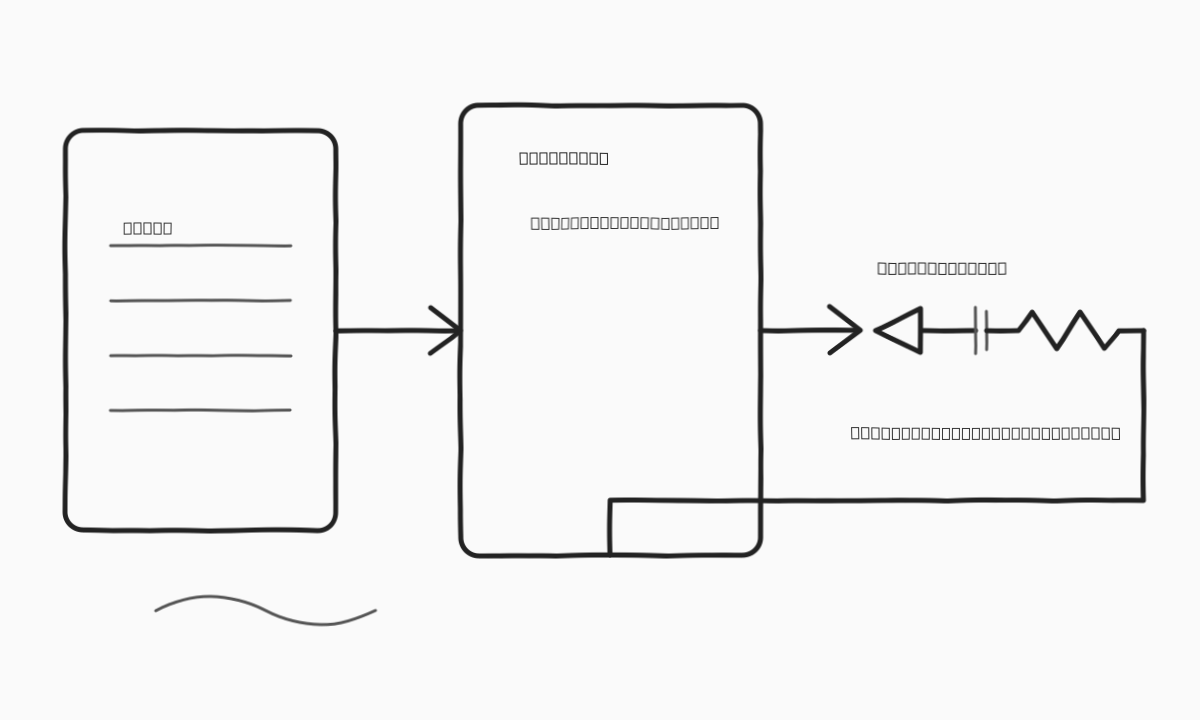
\includegraphics[width=0.96\linewidth]{026-telemetry-packet-pencil.png}

\small\textit{Alternative text: graphite orientation plate showing local
valid, gap, corrupt, and silent fixture packets entering a Mega; the Mega
checks integrity, sequence, and age, then drives one resistor-limited D45
evidence LED. No receiver, antenna, or transmitter is present.}
\end{center}

\section{Exact bounded packet}

The wire image is 19 bytes. It contains no pointer, padding, native enumeration,
native Boolean, or compiler-dependent structure image. Multibyte fields are
big-endian; signed fields use two's-complement bits.

\begin{tabularx}{\linewidth}{@{}r r l X@{}}
\toprule
Offset & Bytes & Field & Meaning\\
\midrule
0 & 1 & magic & \texttt{0xAD}\\
1 & 1 & version & \texttt{0x01}\\
2 & 2 & source ID & opaque lab identifier\\
4 & 2 & sequence & ordering evidence\\
6 & 4 & observed ms & untrusted remote-clock evidence\\
10 & 1 & kind & bounded telemetry kind\\
11 & 1 & quality & bounded sample quality\\
12 & 4 & value & signed integer\\
16 & 1 & exponent & signed decimal scale\\
17 & 2 & CRC-16 & accidental-corruption check\\
\bottomrule
\end{tabularx}

CRC-16/CCITT-FALSE uses polynomial \texttt{0x1021}, initial value
\texttt{0xFFFF}, no reflection, no final XOR, and covers bytes 0--16. It is not
a security primitive.

\texttt{encode()} returns \texttt{Result<uint16\_t>}; callers check
\texttt{ok()} before reading \texttt{value()}. A short output span receives no
partial packet. \texttt{decode()} requires exactly 19 bytes and distinguishes
bad version, length, type, quality, integrity, and trailing data. Failure
leaves the destination unchanged.

\subsection{Packet worksheet}

\begin{tabularx}{\linewidth}{@{}l l X@{}}
\toprule
Check & Prediction & Observation\\
\midrule
Golden valid packet & accepted & \blank{48mm}\\
One changed value bit & bad integrity & \blank{48mm}\\
One byte removed & bad length & \blank{48mm}\\
One byte appended & trailing data & \blank{48mm}\\
Unknown kind & bad type & \blank{48mm}\\
Unknown quality & bad quality & \blank{48mm}\\
\bottomrule
\end{tabularx}

A changed value or timestamp bit with the old CRC reaches
\texttt{BadIntegrity}. A changed magic, version, kind, or quality may reach its
semantic validator first. Tests recompute CRC after a deliberate semantic
change when isolating \texttt{BadVersion}, \texttt{BadType}, or
\texttt{BadQuality}. Every one-bit mutation is rejected; the exact class
follows this precedence.

\section{Sequence is evidence, not arrival order}

The tracker owns one source ID and remembers one accepted observation.
\texttt{First} establishes the baseline. The next sequence is
\texttt{InOrder}; a larger forward jump is \texttt{Gap}. Equal is
\texttt{Duplicate}; evidence behind the accepted value is
\texttt{Reordered}. Comparison uses a documented unsigned half-range rule so
wrap from 65535 to 0 remains deterministic.

The exact delta \texttt{0x8000} is \texttt{Reordered}; it never replaces the
accepted observation.

Duplicate and reordered packets do not replace the accepted sample. A forward
gap may replace it, but the gap remains visible. Source mismatch is invalid
input rather than an observation for a different tracker.

\begin{tabularx}{\linewidth}{@{}r r l X@{}}
\toprule
Accepted & Incoming & State & Does value change?\\
\midrule
--- & 100 & First & yes\\
100 & 101 & InOrder & yes\\
101 & 101 & Duplicate & no\\
101 & 104 & Gap & yes, with gap evidence\\
104 & 103 & Reordered & no\\
65535 & 0 & InOrder & yes, across wrap\\
\bottomrule
\end{tabularx}

Half-range prediction: accepted \blank{18mm}; incoming \blank{18mm};
expected classification \blank{34mm}; reason \blank{55mm}.

\section{Freshness belongs to the receiver}

Age is \texttt{now - receivedAt}, not \texttt{now -
observedMilliseconds}. The remote timestamp is retained for diagnosis, but a
future, reversed, or drifting remote clock cannot keep a packet fresh.

The example uses:
\[
\text{Fresh}<2000\text{ ms},\qquad
2000\leq\text{Aging}<5000\text{ ms},\qquad
\text{Stale}\geq5000\text{ ms}.
\]

\begin{tabularx}{\linewidth}{@{}r l l@{}}
\toprule
Local age & Prediction & Observation\\
\midrule
1999 ms & Fresh & \blank{45mm}\\
2000 ms & Aging & \blank{45mm}\\
4999 ms & Aging & \blank{45mm}\\
5000 ms & Stale & \blank{45mm}\\
\bottomrule
\end{tabularx}

Now reverse the packet's remote timestamp while keeping the same local receipt
time.

Prediction: \blank{90mm}.

Interpretation: \blank{95mm}.

\section{Narrative run loop and visible state}

\begin{lstlisting}[style=adkcpp]
observePacket           (now);
verifyPacket            (now);
updateFreshness         (now);
showObservationEvidence (now);
\end{lstlisting}

Objects appear in dependency order: runtime, acquisition LED, packet-evidence
LED, pure codec, then tracker. Setup acquires, configures, and starts. The loop
observes one scheduled fixture, verifies exact packet bytes, updates freshness,
and actuates D45.

The 12-second schedule accepts sequence 1, skips 2 and accepts 3, corrupts the
next packet, waits until sequence 3 becomes stale, then accepts sequence 4
after wrap. Every advertised evidence state is reachable, and recovery is an
accepted in-order observation rather than a display reset.

\texttt{TelemetryFixtureSchedule} owns this tested one-shot decision trace; the
sketch does not duplicate its timing policy. \texttt{TelemetryEvidenceModel}
applies the tested precedence fault, corrupt, stale, sequence/aging, then
fresh. The four run-loop calls therefore name actual work rather than
forwarding into another private state machine. An unexpected execution fault
uses the safe-off path; the four-pulse fixture demonstrates corrupt packet
evidence, not a claim that a failed output can diagnose itself.

\begin{tabularx}{\linewidth}{@{}l l X@{}}
\toprule
State & D45 cadence & Meaning\\
\midrule
Fresh, in order & one 1 s pulse & accepted observation is fresh\\
Sequence or aging & two 150 ms pulses & duplicate, gap, reorder, or aging\\
Stale & three 120 ms pulses & no recent accepted observation\\
Corrupt fixture & four 100 ms pulses & packet integrity failed\\
\bottomrule
\end{tabularx}

D13 proves acquisition only. D45 reports current evidence only. Serial may
print supporting records, but it does not control tuning, capture, or replay
and is never the sole observation.

\section{Predict, observe, interpret}

\subsection{Experiment A: acquisition}

\textbf{Predict.} D13 illuminates only after the tracker and both output
endpoints initialize.

\textbf{Observe:} \blank{90mm}.
\textbf{Interpret.} This supports acquisition, not packet correctness or safe
shutdown.

\subsection{Experiment B: deterministic fixture cycle}

Before upload, predict each D45 cadence. Probe TP-LED against GND and record:

\begin{tabularx}{\linewidth}{@{}l l l l@{}}
\toprule
Fixture & Predicted count & Observed count & Pulse widths\\
\midrule
valid & \blank{18mm} & \blank{18mm} & \blank{30mm}\\
forward gap & \blank{18mm} & \blank{18mm} & \blank{30mm}\\
corrupt & \blank{18mm} & \blank{18mm} & \blank{30mm}\\
silence to stale & \blank{18mm} & \blank{18mm} & \blank{30mm}\\
\bottomrule
\end{tabularx}

Agreement supports the path from fixture bytes through integrity, tracker, and
visible actuation. It proves no RF, network, remote sensor, or security claim.

\subsection{Experiment C: safe state}

Invoke shutdown. Predict D13 and D45 inactive and both pins released. Observe
the LEDs, then measure TP-LED separately. A dark LED does not prove high
impedance or claim release.

Measured safe-state evidence: \blank{80mm}.

\section{Diagnosis and privacy review}

\begin{tabularx}{\linewidth}{@{}l X@{}}
\toprule
Observation & Check next\\
\midrule
D13 dark & tracker configuration, output claim conflict, board power\\
D13 on; D45 dark & fixture schedule, LED polarity, resistor, TP-LED\\
valid becomes corrupt & exact length, version, byte order, CRC coverage\\
gap never appears & sequence fixture and half-range comparison\\
stale never appears & local receipt time and exact 5 s boundary\\
state changes from remote clock & defect: freshness must use local receipt\\
D45 driven after stop & safe-state failure; remove USB and record deviation\\
\bottomrule
\end{tabularx}

\subsection{Minimum-data worksheet}

For every proposed field ask: Does the experiment require it? Could it identify
a person, place, account, or device? Can an opaque lab identifier replace it?
How long must it be retained?

\begin{tabularx}{\linewidth}{@{}l l l X@{}}
\toprule
Proposed field & Required? & Opaque substitute? & Retention reason\\
\midrule
\blank{28mm} & \blank{16mm} & \blank{25mm} & \blank{38mm}\\
\blank{28mm} & \blank{16mm} & \blank{25mm} & \blank{38mm}\\
\blank{28mm} & \blank{16mm} & \blank{25mm} & \blank{38mm}\\
\bottomrule
\end{tabularx}

Use only owned lab fixtures. Do not collect device serial numbers, addresses,
locations, credentials, or unnecessary payloads. This lesson contains no
receiver, transmitter, raw capture export, rolling-code analysis, key
recovery, replay, or command mapping.

\section{CLI and open acceptance records}

\begin{verbatim}
make host-test
make arduino-Lesson026TelemetryPacket
make size-Lesson026TelemetryPacket
make upload-Lesson026TelemetryPacket PORT=/dev/ttyACM0
make serial-log PORT=/dev/ttyACM0
make lessons
make lessons-check
make site-check
\end{verbatim}

\textbf{Software fixture acceptance}

\begin{itemize}
  \item \checkbox\ Golden valid packet and exact encoded bytes compared.
  \item \checkbox\ All one-bit corruption positions rejected by host tests.
  \item \checkbox\ Truncation, extension, unaligned input, and short output tested.
  \item \checkbox\ Sequence first/in-order/duplicate/gap/reorder/wrap tested.
  \item \checkbox\ Freshness edges and remote-clock independence tested.
  \item \checkbox\ Identical fixtures and receipt times replay byte identically.
\end{itemize}

Commit \blank{34mm}; compiler \blank{30mm}; result \blank{40mm}.

\textbf{Mega bench acceptance---open until measured}

\begin{itemize}
  \item \checkbox\ Exact Mega, LED, resistor, supply, and instrument recorded.
  \item \checkbox\ Unpowered D45 wiring and polarity checked.
  \item \checkbox\ D13 acquisition evidence observed separately.
  \item \checkbox\ One-, two-, three-, and four-pulse patterns measured.
  \item \checkbox\ TP-LED widths and periods recorded against GND.
  \item \checkbox\ Reset, shutdown, USB removal, and claim reuse observed.
  \item \checkbox\ D45 safe state checked separately from LED appearance.
\end{itemize}

Supply \blank{20mm}; instrument \blank{34mm}; date \blank{22mm};
reviewer \blank{30mm}. Deviations: \blank{70mm}.

\lessonbox{\textbf{Current result: host verified; hardware acceptance open.}
Fixtures, compilation, and blank worksheets are not physical verification.}

\section{Exercises and further reading}

\begin{enumerate}
  \item Change each bit of one golden packet in turn. Explain why rejection
        establishes error detection but not sender identity.
  \item Prove that a one-byte-short encoder destination remains unchanged.
  \item Draw the five sequence classes around 16-bit wrap and half range.
  \item Make the remote timestamp move backward while local time advances.
        Predict freshness before running the test.
  \item Propose a minimal humidity sample record. Remove every field that the
        experiment does not need.
  \item Explain why sample quality \texttt{SensorFault}, transport corruption,
        and local staleness must remain three different observations.
\end{enumerate}

\begin{itemize}
  \item
    \href{https://spincyc.github.io/adk/lessons/026.html}
         {HTML reference and corrections}
  \item
    \href{https://github.com/spincyc/adk/blob/main/src/telemetry_packet.h}
         {TelemetryPacketCodec public header} and
    \href{https://github.com/spincyc/adk/blob/main/src/telemetry_packet.cpp}
         {implementation}
  \item
    \href{https://github.com/spincyc/adk/blob/main/tests/test_telemetry_packet.cpp}
         {packet golden-vector and corruption tests}
  \item
    \href{https://github.com/spincyc/adk/blob/main/src/observation_tracker.h}
         {ObservationTracker public header} and
    \href{https://github.com/spincyc/adk/blob/main/src/observation_tracker.cpp}
         {implementation}
  \item
    \href{https://github.com/spincyc/adk/blob/main/tests/test_observation_tracker.cpp}
         {tracker lifecycle and timing tests}
  \item
    \href{https://github.com/spincyc/adk/blob/main/src/telemetry_evidence.h}
         {fixture schedule and evidence model} and
    \href{https://github.com/spincyc/adk/blob/main/tests/test_telemetry_evidence.cpp}
         {fixture and visible-precedence tests}
  \item
    \href{https://github.com/spincyc/adk/blob/main/docs/design/LESSONS_025_027_TELEMETRY.md}
         {Lessons 025--027 executable design}
  \item
    \href{https://docs.arduino.cc/resources/datasheets/A000067-datasheet.pdf}
         {Arduino Mega 2560 Rev3 datasheet}
\end{itemize}

\end{document}
